\documentclass[UTF8]{article}

\usepackage{amsmath, amsfonts, amssymb, amstext, amscd, amsthm, bbm, CJKutf8, color, dsfont, enumerate, float, graphicx, hyperref, makeidx, mathrsfs, mathtools, marvosym, soul, url, verbatim, xcolor, xfrac}
\usepackage[left=2cm,top=2cm,right=2cm,bottom=2cm,bindingoffset=0cm]{geometry}
\allowdisplaybreaks 
\newenvironment{subproof}[1][Proof]
    {\proof[#1]\leftskip=1cm\rightskip=1cm}
	{\endproof}

%theorems with custom numbering
%\newtheorem{innerthm}{Theorem}
%\newenvironment{thm}[1]
    %{\renewcommand\theinnerthm{#1}\innercustomthm}
    %{\endinnerthm}

\newtheorem{theorem}{Theorem}
\newtheorem{lemma}{Lemma}
\newtheorem{proposition}{Proposition}
\newtheorem{corollary}{Corollary}
\newtheorem{claim}{Claim}
\newtheorem{conjecture}{Conjecture}
\newtheorem{justification}{Justification}
\newtheorem{definition}{Definition}
\newtheorem*{remark}{Remark}
\newtheorem*{note}{Note}

\renewcommand{\and}{\;\wedge\;}
\newcommand{\disj}{\;\vee\;}
\newcommand{\xor}{\;\oplus\;}
\newcommand{\divides}{\;|\;}
\newcommand{\suchthat}{\;\middle|\;}
\newcommand{\contradiction}{\;\text{\Large \Lightning}}
\newcommand{\conj}[1]{\overline{#1}}
\newcommand{\mean}[1]{\overline{#1}}
\newcommand{\integral}[1]{\smashoperator{\int_{#1}}}
\renewcommand{\restriction}[1]{\downharpoonright_{#1}}
\renewcommand{\qedsymbol}{QED}

\DeclareMathOperator{\lcm}{lcm}
\DeclareMathOperator*{\argmin}{arg\!\min}
\DeclareMathOperator*{\argmax}{arg\!\max}

\let\originalleft\left
\let\originalright\right
\renewcommand{\left}{\mathopen{}\mathclose\bgroup\originalleft}
\renewcommand{\right}{\aftergroup\egroup\originalright}
\newcommand{\zh}[1]{\begin{CJK}{UTF8}{gbsn}#1\end{CJK}}
\newcommand{\jp}[1]{\begin{CJK}{UTF8}{gbsn}#1\end{CJK}}

\DeclarePairedDelimiterX \inner[2]{\langle}{\rangle}{#1,#2}
\DeclarePairedDelimiterX \braket[2]{\langle}{\rangle}{#1 \delimsize\vert #2}
\DeclarePairedDelimiter \bra{\langle}{\rvert}
\DeclarePairedDelimiter \ket{\lvert}{\rangle}
\DeclarePairedDelimiter \abs{\lvert}{\rvert}
\DeclarePairedDelimiter \lrangle{\langle}{\rangle}
\DeclarePairedDelimiter \norm{\lVert}{\rVert}
\DeclarePairedDelimiter \set{\lbrace}{\rbrace}
\DeclarePairedDelimiter \parens{(}{)}

\begin{document}
\begin{center}
	\textsc{\huge Applied Machine Learning}\\
	\textsc{\Large Homework 4}\\
\end{center}
\begin{flushright}
	Daniel Gonzalez\\
    Colton Piper\\
	$26^{\text{th}}$ of September, $2018$
\end{flushright}


\section{Results}
After speaking with Prof. Barbu, we decided to use $w_0$ in our computations, along with a column of $1$s in our data matrix,
since Prof. Barbu made the argument that ignoring $w_0$ removes one degree of freedom from our model and would give worse generalization for the classifier.
However, the important thing to note is that $w_0$ is does not undergo thresholding via $\Theta$, since we are not treating $w_0$ like a feature for selection.
When comparing our results to results we'd previously computed ignoring $w_0$, our misclassification errors were slightly lower,
but not low enough to be noticeable on a graph or to be worth tabulating.

For this entire assignment, we used $\eta = \sfrac{1}{N}$ where $N$ is the number of samples in the training data.

\subsection{Table}

\begin{table}[H]
\centering
    \caption{Summary of Results}
    \begin{tabular}{|l|l|l|l|l|}
        \hline
        \texttt{\# Data Set}&\multicolumn{1}{|c|}{$\lambda$}&\texttt{Features Selected}&\texttt{Training Error}&\texttt{Test Error}\\\hline
        \texttt{gisette} & $0.197$ & $10$ & $11.4833\dots\%$ & $10.4\%$\\\cline{2-5}
         & $0.134$ & $30$ & $6.6\%$ & $7.3\%$\\\cline{2-5}
         & $0.08745$ & $100$ & $3.1\%$ & $3.3\%$\\\cline{2-5}
         & $0.053$ & $300$ & $1.25\%$ & $1.8\%$\\\hline\cline{1-5}

        \texttt{dexter} & $0.15$ & $10$ & $15.6666\dots\%$ & $18.0\%$\\\cline{2-5}
         & $0.0983663$ & $31$ & $5.0\%$ & $12.0\%$\\\cline{2-5}
         & $0.0713$ & $100$ & $1.6666\dots\%$ & $8.0\%$\\\cline{2-5}
         & $0.05269$ & $293$ & $0.0\%$ & $6.6666\dots\%$\\\hline\cline{1-5}

        \texttt{madelon} & $0.029799$ & $8$ & $38.6\%$ & $39.5\%$\\\cline{2-5}
         & $0.02435$ & $30$ & $35.7\%$ & $42.8333\dots\%$\\\cline{2-5}
         & $0.01695$ & $100$ & $32.6\%$ & $42.8333\dots\%$\\\cline{2-5}
         & $0.0074$ & $299$ & $27.05\%$ & $42.8333\dots\%$\\\hline
    \end{tabular}
\end{table}

\subsection{Figures}
\begin{figure}[H]
    \centering
    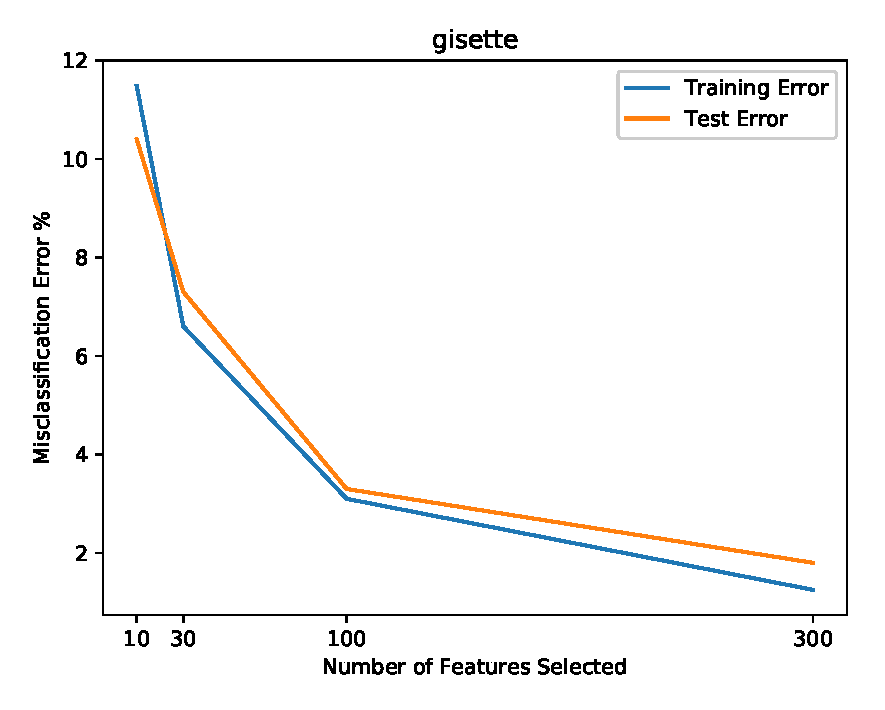
\includegraphics[scale=0.95]{./figures/gisette.eps}
\end{figure}

\begin{figure}[H]
    \centering
    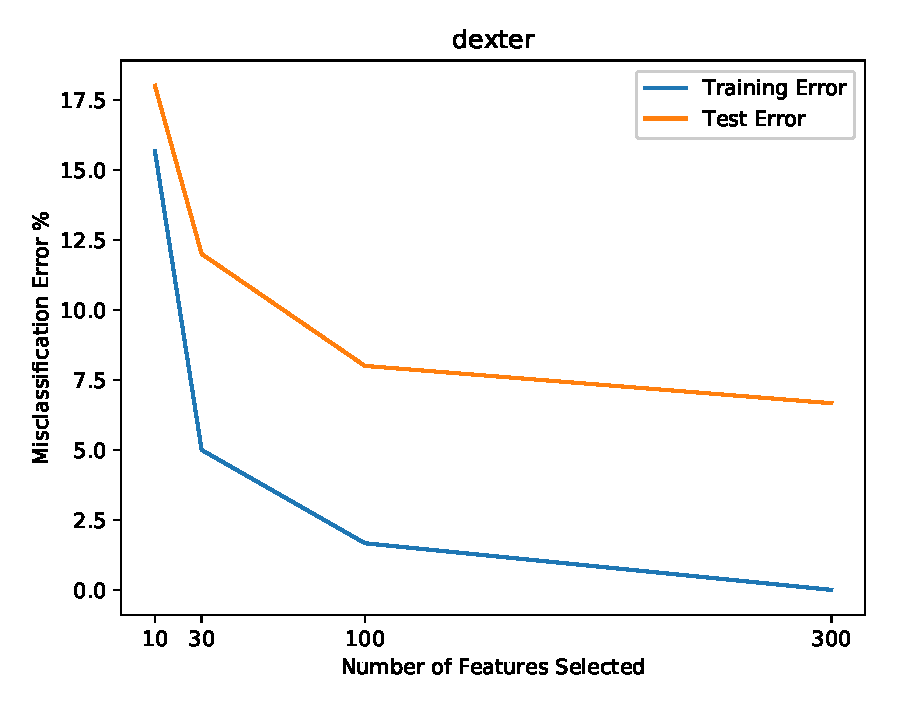
\includegraphics[scale=0.95]{./figures/dexter.eps}
\end{figure}

\begin{figure}[H]
    \centering
    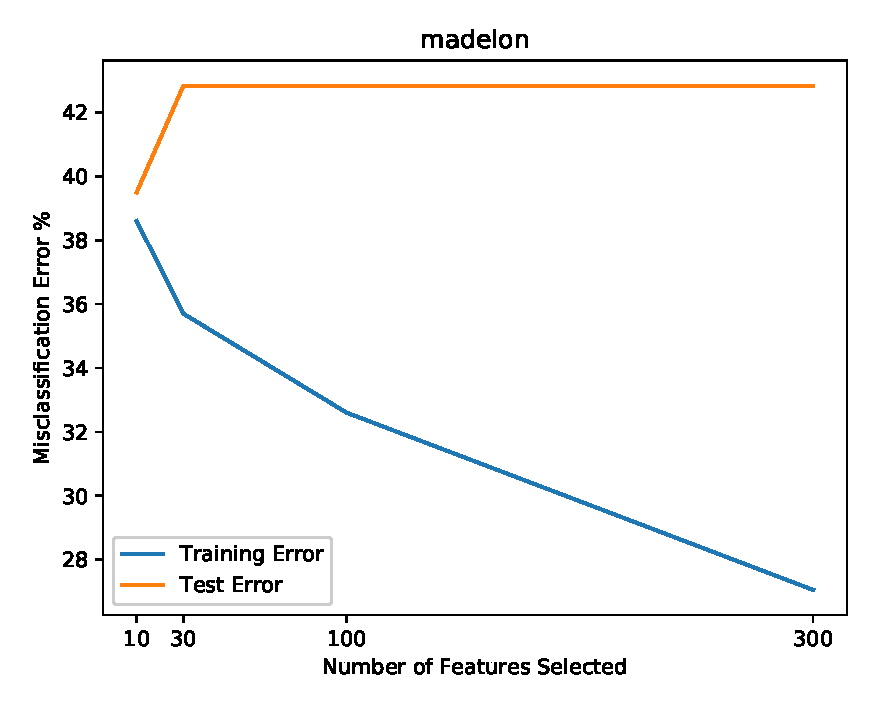
\includegraphics[scale=0.95]{./figures/madelon.eps}
\end{figure}

\newpage
\section{Appendix: Code}
If the code looks too small, please zoom in on the pdf.
The screenshots are \texttt{.png} images, so you should be able to zoom in and read at whatever is a comfortable size for you.
\begin{figure}[H]
    \centering
    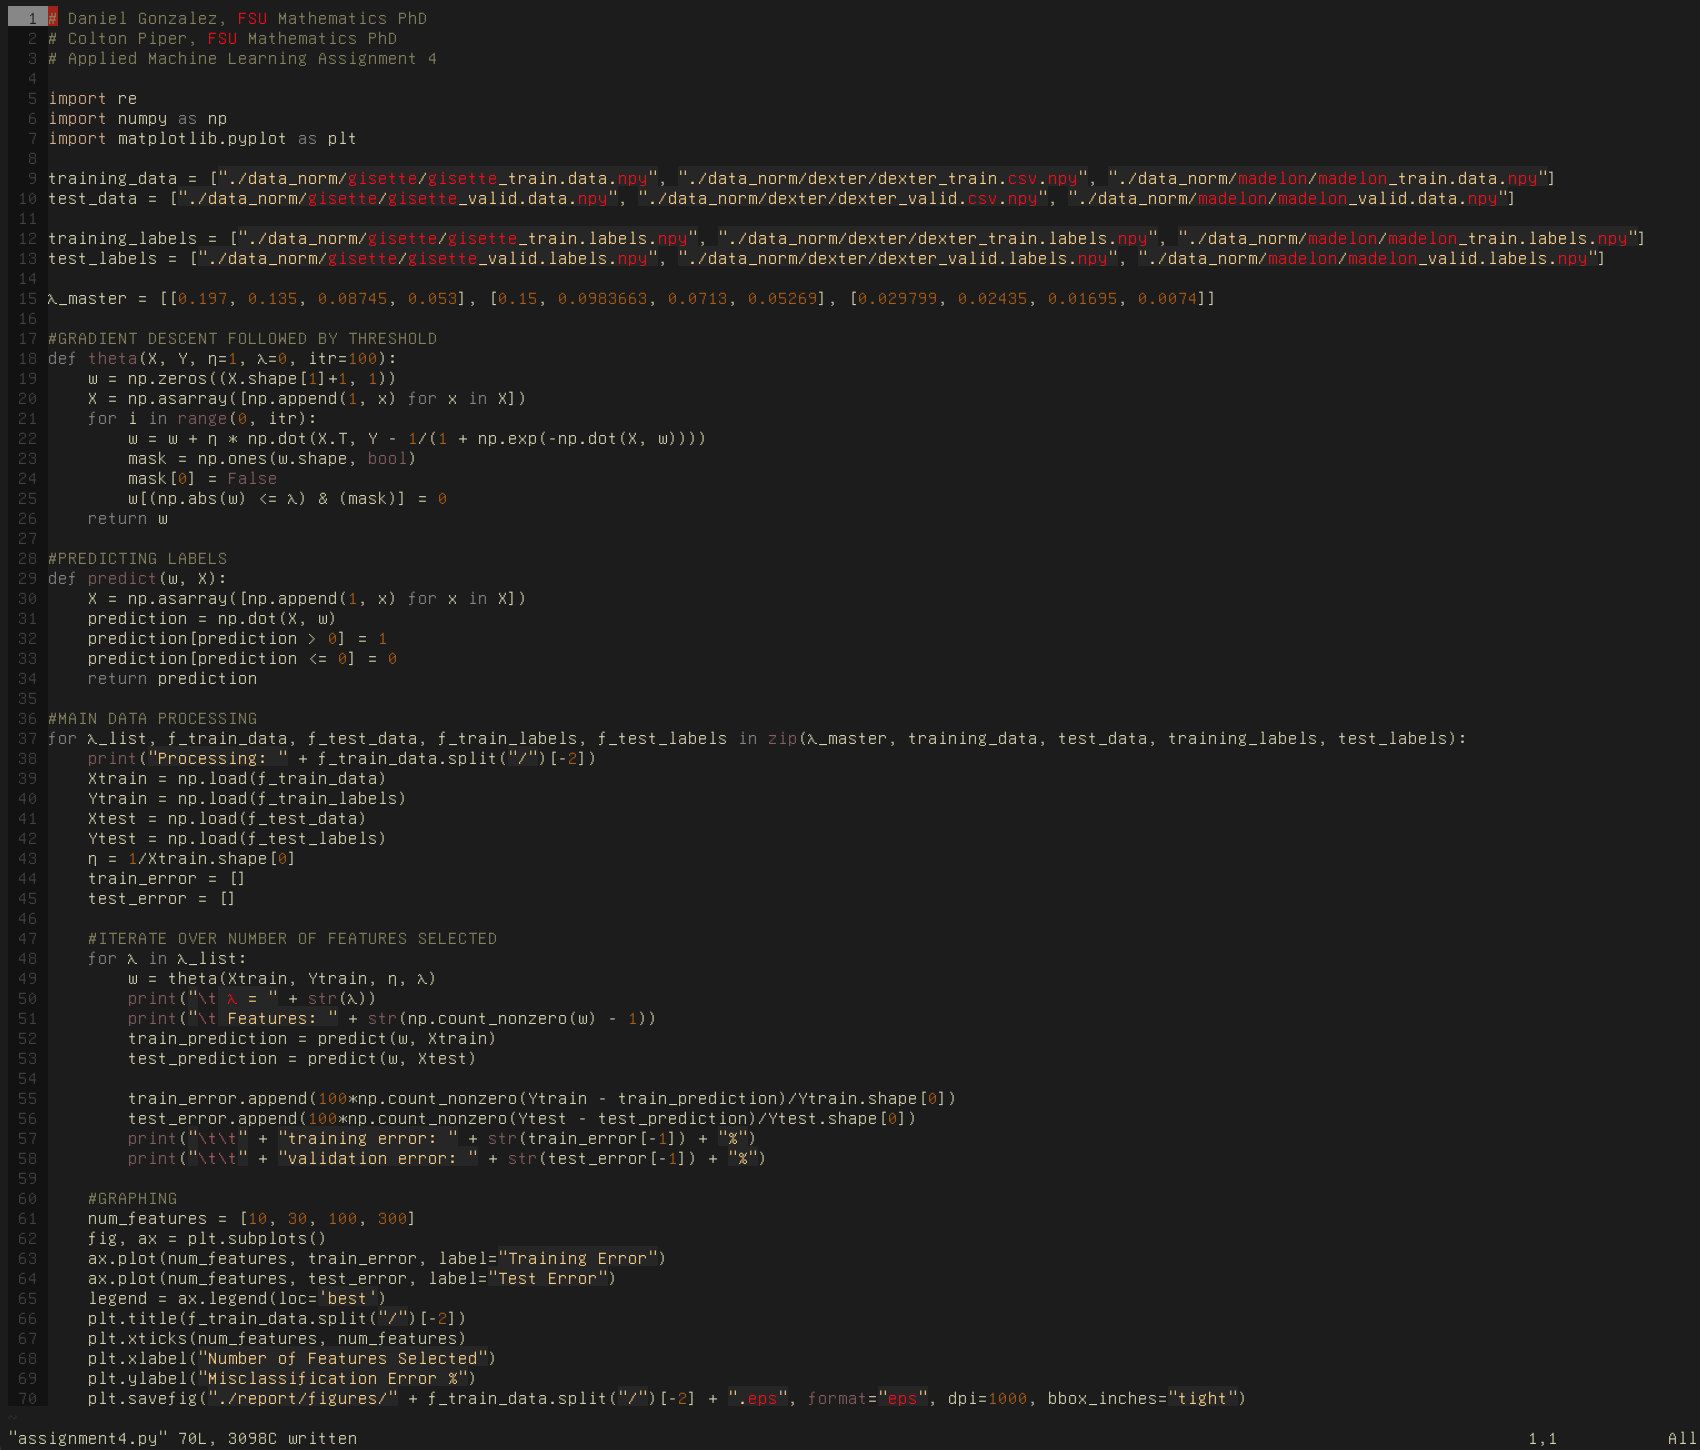
\includegraphics[scale=0.6]{./figures/code_TISP.png}
\end{figure}
\begin{figure}[H]
    \centering
    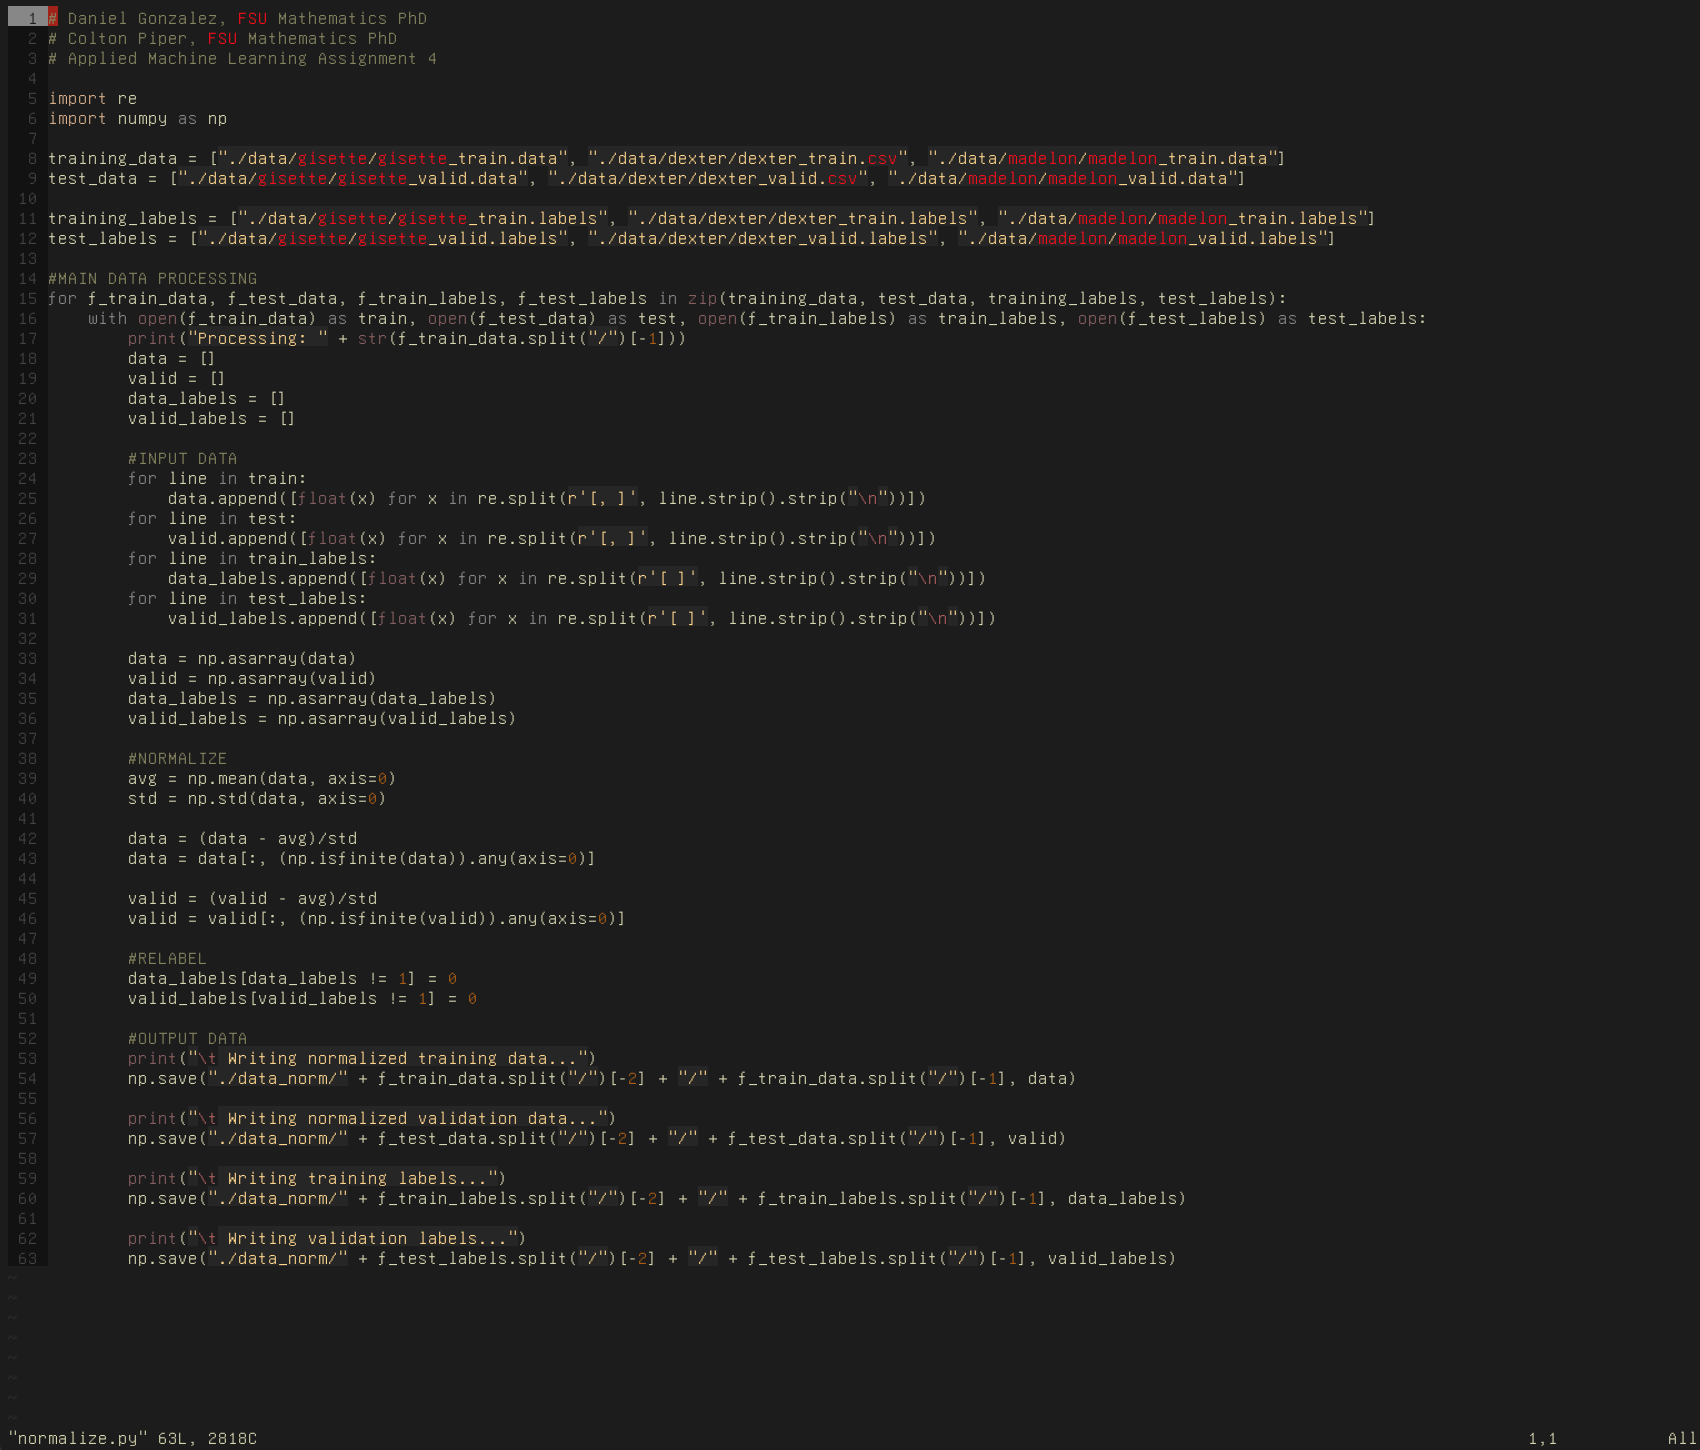
\includegraphics[scale=0.6]{./figures/code_normalize.png}
\end{figure}

\end{document}
